% Options for packages loaded elsewhere
\PassOptionsToPackage{unicode}{hyperref}
\PassOptionsToPackage{hyphens}{url}
%
\documentclass[
]{article}
\usepackage{amsmath,amssymb}
\usepackage{lmodern}
\usepackage{iftex}
\ifPDFTeX
  \usepackage[T1]{fontenc}
  \usepackage[utf8]{inputenc}
  \usepackage{textcomp} % provide euro and other symbols
\else % if luatex or xetex
  \usepackage{unicode-math}
  \defaultfontfeatures{Scale=MatchLowercase}
  \defaultfontfeatures[\rmfamily]{Ligatures=TeX,Scale=1}
\fi
% Use upquote if available, for straight quotes in verbatim environments
\IfFileExists{upquote.sty}{\usepackage{upquote}}{}
\IfFileExists{microtype.sty}{% use microtype if available
  \usepackage[]{microtype}
  \UseMicrotypeSet[protrusion]{basicmath} % disable protrusion for tt fonts
}{}
\makeatletter
\@ifundefined{KOMAClassName}{% if non-KOMA class
  \IfFileExists{parskip.sty}{%
    \usepackage{parskip}
  }{% else
    \setlength{\parindent}{0pt}
    \setlength{\parskip}{6pt plus 2pt minus 1pt}}
}{% if KOMA class
  \KOMAoptions{parskip=half}}
\makeatother
\usepackage{xcolor}
\usepackage[margin=1in]{geometry}
\usepackage{color}
\usepackage{fancyvrb}
\newcommand{\VerbBar}{|}
\newcommand{\VERB}{\Verb[commandchars=\\\{\}]}
\DefineVerbatimEnvironment{Highlighting}{Verbatim}{commandchars=\\\{\}}
% Add ',fontsize=\small' for more characters per line
\usepackage{framed}
\definecolor{shadecolor}{RGB}{248,248,248}
\newenvironment{Shaded}{\begin{snugshade}}{\end{snugshade}}
\newcommand{\AlertTok}[1]{\textcolor[rgb]{0.94,0.16,0.16}{#1}}
\newcommand{\AnnotationTok}[1]{\textcolor[rgb]{0.56,0.35,0.01}{\textbf{\textit{#1}}}}
\newcommand{\AttributeTok}[1]{\textcolor[rgb]{0.77,0.63,0.00}{#1}}
\newcommand{\BaseNTok}[1]{\textcolor[rgb]{0.00,0.00,0.81}{#1}}
\newcommand{\BuiltInTok}[1]{#1}
\newcommand{\CharTok}[1]{\textcolor[rgb]{0.31,0.60,0.02}{#1}}
\newcommand{\CommentTok}[1]{\textcolor[rgb]{0.56,0.35,0.01}{\textit{#1}}}
\newcommand{\CommentVarTok}[1]{\textcolor[rgb]{0.56,0.35,0.01}{\textbf{\textit{#1}}}}
\newcommand{\ConstantTok}[1]{\textcolor[rgb]{0.00,0.00,0.00}{#1}}
\newcommand{\ControlFlowTok}[1]{\textcolor[rgb]{0.13,0.29,0.53}{\textbf{#1}}}
\newcommand{\DataTypeTok}[1]{\textcolor[rgb]{0.13,0.29,0.53}{#1}}
\newcommand{\DecValTok}[1]{\textcolor[rgb]{0.00,0.00,0.81}{#1}}
\newcommand{\DocumentationTok}[1]{\textcolor[rgb]{0.56,0.35,0.01}{\textbf{\textit{#1}}}}
\newcommand{\ErrorTok}[1]{\textcolor[rgb]{0.64,0.00,0.00}{\textbf{#1}}}
\newcommand{\ExtensionTok}[1]{#1}
\newcommand{\FloatTok}[1]{\textcolor[rgb]{0.00,0.00,0.81}{#1}}
\newcommand{\FunctionTok}[1]{\textcolor[rgb]{0.00,0.00,0.00}{#1}}
\newcommand{\ImportTok}[1]{#1}
\newcommand{\InformationTok}[1]{\textcolor[rgb]{0.56,0.35,0.01}{\textbf{\textit{#1}}}}
\newcommand{\KeywordTok}[1]{\textcolor[rgb]{0.13,0.29,0.53}{\textbf{#1}}}
\newcommand{\NormalTok}[1]{#1}
\newcommand{\OperatorTok}[1]{\textcolor[rgb]{0.81,0.36,0.00}{\textbf{#1}}}
\newcommand{\OtherTok}[1]{\textcolor[rgb]{0.56,0.35,0.01}{#1}}
\newcommand{\PreprocessorTok}[1]{\textcolor[rgb]{0.56,0.35,0.01}{\textit{#1}}}
\newcommand{\RegionMarkerTok}[1]{#1}
\newcommand{\SpecialCharTok}[1]{\textcolor[rgb]{0.00,0.00,0.00}{#1}}
\newcommand{\SpecialStringTok}[1]{\textcolor[rgb]{0.31,0.60,0.02}{#1}}
\newcommand{\StringTok}[1]{\textcolor[rgb]{0.31,0.60,0.02}{#1}}
\newcommand{\VariableTok}[1]{\textcolor[rgb]{0.00,0.00,0.00}{#1}}
\newcommand{\VerbatimStringTok}[1]{\textcolor[rgb]{0.31,0.60,0.02}{#1}}
\newcommand{\WarningTok}[1]{\textcolor[rgb]{0.56,0.35,0.01}{\textbf{\textit{#1}}}}
\usepackage{graphicx}
\makeatletter
\def\maxwidth{\ifdim\Gin@nat@width>\linewidth\linewidth\else\Gin@nat@width\fi}
\def\maxheight{\ifdim\Gin@nat@height>\textheight\textheight\else\Gin@nat@height\fi}
\makeatother
% Scale images if necessary, so that they will not overflow the page
% margins by default, and it is still possible to overwrite the defaults
% using explicit options in \includegraphics[width, height, ...]{}
\setkeys{Gin}{width=\maxwidth,height=\maxheight,keepaspectratio}
% Set default figure placement to htbp
\makeatletter
\def\fps@figure{htbp}
\makeatother
\setlength{\emergencystretch}{3em} % prevent overfull lines
\providecommand{\tightlist}{%
  \setlength{\itemsep}{0pt}\setlength{\parskip}{0pt}}
\setcounter{secnumdepth}{-\maxdimen} % remove section numbering
\ifLuaTeX
  \usepackage{selnolig}  % disable illegal ligatures
\fi
\IfFileExists{bookmark.sty}{\usepackage{bookmark}}{\usepackage{hyperref}}
\IfFileExists{xurl.sty}{\usepackage{xurl}}{} % add URL line breaks if available
\urlstyle{same} % disable monospaced font for URLs
\hypersetup{
  pdftitle={HARP AT METEO-ALGERIA},
  pdfauthor={CHIKHI Walid},
  hidelinks,
  pdfcreator={LaTeX via pandoc}}

\title{HARP AT METEO-ALGERIA}
\author{CHIKHI Walid}
\date{Avril 2022}

\begin{document}
\maketitle

{
\setcounter{tocdepth}{2}
\tableofcontents
}
\hypertarget{pruxe9sentation-harp}{%
\subsection{Présentation Harp}\label{pruxe9sentation-harp}}

HARP est un outil pour lire, traiter et comparer les données de
télédétection par satellite, les données de modèle, les données in situ
et les données de télédétection au sol. Cet outil est composé de :

\begin{itemize}
\tightlist
\item
  Un ensemble d'outils de ligne de commande
\item
  Une bibliothèque de fonctions d'analyse
\end{itemize}

Harp en considération plusieurs formats de données : (NetCDF - HDF5 - FA
- LFI - GRIB) et peut étre manipulé en utilisant R , Python - Matlab -
IDL ou des lignes de commandes UNIX¨.

Ce document présente un guide pour débutant harp afin de l'installer et
l'utiliser sur Rstudio.

\hypertarget{installation-harp-sur-r}{%
\subsection{Installation harp sur R}\label{installation-harp-sur-r}}

le package Harp n'est pas disponible sur le repertoire CRAN du Langage
R, Pour cela une installation directe du github sera menée.avant
d'entamer l'installation nous devons dabord installer les prérequis :

\begin{Shaded}
\begin{Highlighting}[]
\CommentTok{\#install.packages("devtools")}
\CommentTok{\#install.packages("tydiverse")}
\CommentTok{\#install.packages("tinytex")}
\end{Highlighting}
\end{Shaded}

Maintenant procédons a l'installation du package harp Basic (ne prend
pas en considération les formats LFI et FA ) \^{} :

\begin{Shaded}
\begin{Highlighting}[]
\CommentTok{\# Installation de HARP }

\CommentTok{\#library(devtools)}
\CommentTok{\#install\_github("harphub/harp", force = TRUE)}
\end{Highlighting}
\end{Shaded}

Si l'installation du package a été effectué avec succés un message de ce
genre sera affiché sur la console de Rstudio :

\begin{center}\rule{0.5\linewidth}{0.5pt}\end{center}

\begin{verbatim}
## Le chargement a nécessité le package : usethis
\end{verbatim}

\begin{center}\rule{0.5\linewidth}{0.5pt}\end{center}

Afin d'utiliser un package sur R , nous devons tous dabord le charger
sur notre environnement de travail. la fonction \textbf{library()} de R
permets de faire cela:

\begin{Shaded}
\begin{Highlighting}[]
\CommentTok{\# library(tinytex)}
\CommentTok{\# library(harp)}
\end{Highlighting}
\end{Shaded}

\hypertarget{comment-travailler-avec-les-formats-lfi-et-fa}{%
\subsection{Comment Travailler avec les formats LFI et
FA}\label{comment-travailler-avec-les-formats-lfi-et-fa}}

Bien que les sorties des modéles opérationels utilisés au sein de
Météo-Algérie soient du format ``LFI'' et ``FA'' ou plus couramment
nommée par le services de la PNT ``Fullpos'' et ``ICMSH'', le package de
base harp ne prend ces deux format en compte, et pour de raisons de
confidentialité le code source du package \emph{``Rfa''} pour la
manipulation de ces 2 formats n'est pas publiquement paratgé jusqu'a
présent sur aucun service web. Pour se procurer le package Rfa , vous
devriez contacter Monsieur \textbf{\emph{Alex} \emph{Deckmyn}}
\textless{}
\emph{\href{mailto:alex.deckmyn@meteo.be}{\nolinkurl{alex.deckmyn@meteo.be}}}
\textgreater{} du l'institut Royal de Météorologie (IRM)

\hypertarget{guide-dutilisation}{%
\subsection{\texorpdfstring{\emph{Guide
d'utilisation}}{Guide d'utilisation}}\label{guide-dutilisation}}

Ce chapitre est en cours d'exploration.

\hypertarget{exemple}{%
\paragraph{\texorpdfstring{\emph{Exemple}}{Exemple}}\label{exemple}}

Voici un petit exemple pour la manipulation d'un fichier FA

\begin{Shaded}
\begin{Highlighting}[]
\FunctionTok{library}\NormalTok{(Rfa)}
\end{Highlighting}
\end{Shaded}

\begin{verbatim}
## Le chargement a nécessité le package : meteogrid
\end{verbatim}

\begin{Shaded}
\begin{Highlighting}[]
\FunctionTok{library}\NormalTok{(harp)}
\end{Highlighting}
\end{Shaded}

\begin{verbatim}
## Le chargement a nécessité le package : harpIO
\end{verbatim}

\begin{verbatim}
## Le chargement a nécessité le package : harpPoint
\end{verbatim}

\begin{verbatim}
## Le chargement a nécessité le package : harpVis
\end{verbatim}

\begin{verbatim}
## Le chargement a nécessité le package : ggplot2
\end{verbatim}

\begin{verbatim}
## Le chargement a nécessité le package : shiny
\end{verbatim}

\begin{verbatim}
## Le chargement a nécessité le package : harpSpatial
\end{verbatim}

\begin{Shaded}
\begin{Highlighting}[]
\CommentTok{\# Lire un champ a partir d\textquotesingle{}un ICMSH et l\textquotesingle{}attribuer a un variable. }

\NormalTok{t2m}\OtherTok{=}\NormalTok{Rfa}\SpecialCharTok{::}\FunctionTok{FAdec}\NormalTok{(}\StringTok{"\textasciitilde{}/Dropbox/Harp/PFAL03ALGE01+0000"}\NormalTok{,}\StringTok{"SURFTEMPERATURE"}\NormalTok{)}
\FunctionTok{plot\_field}\NormalTok{(t2m)}
\end{Highlighting}
\end{Shaded}

\begin{verbatim}
## Nothing to project!
## Nothing to project!
## Nothing to project!
## Nothing to project!
## Nothing to project!
## Nothing to project!
\end{verbatim}

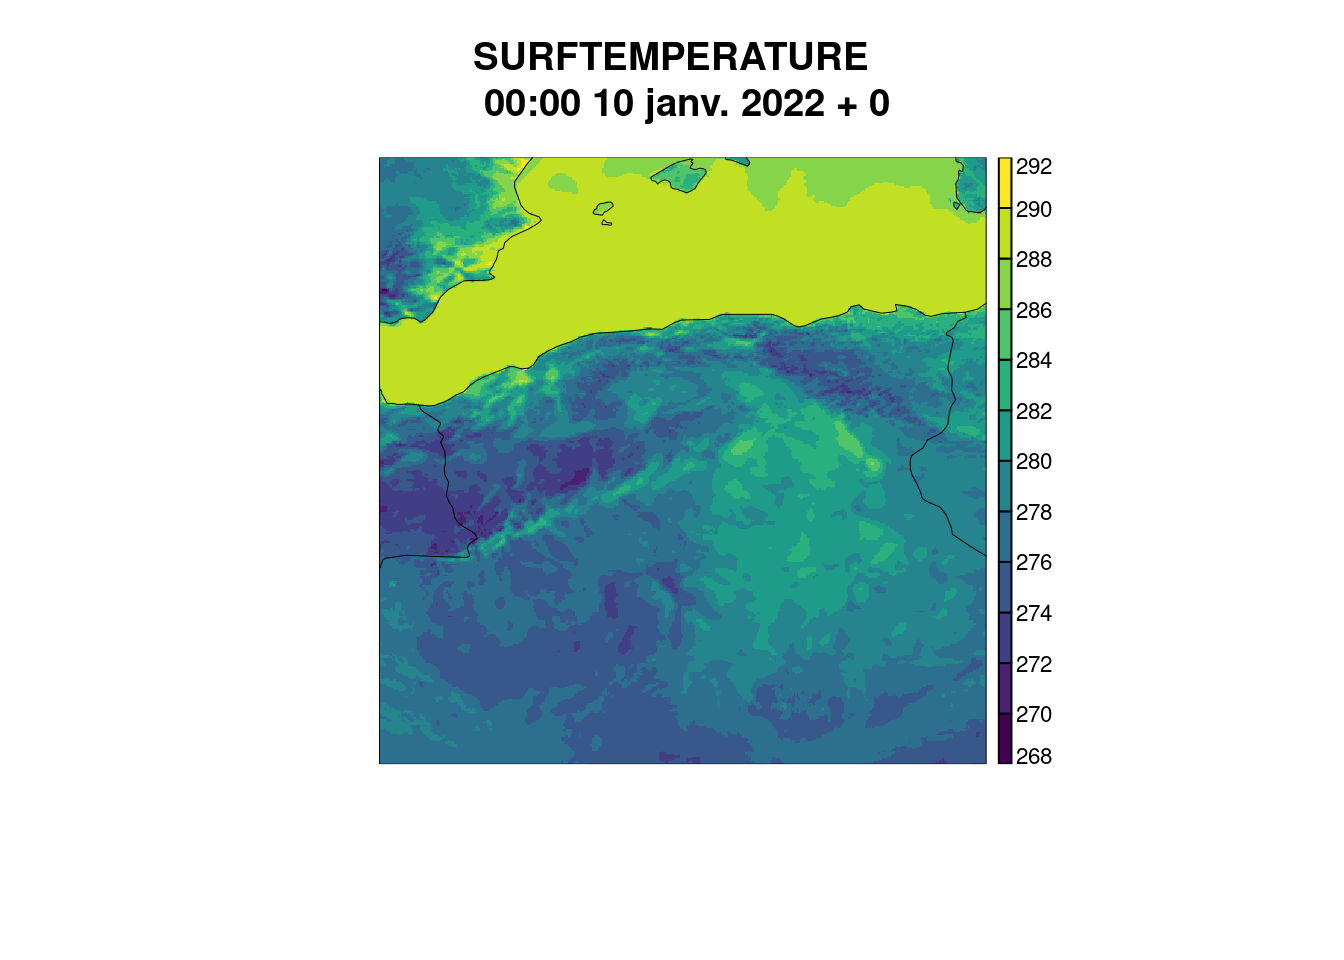
\includegraphics{harp_files/figure-latex/unnamed-chunk-5-1.pdf}

\begin{verbatim}
## Nothing to project!
## Nothing to project!
## Nothing to project!
## Nothing to project!
## Nothing to project!
## Nothing to project!
## Nothing to project!
## Nothing to project!
## Nothing to project!
## Nothing to project!
## Nothing to project!
## Nothing to project!
## Nothing to project!
\end{verbatim}

\hypertarget{lire-une-pruxe9vision-avec-harp}{%
\subsection{Lire une prévision avec
Harp}\label{lire-une-pruxe9vision-avec-harp}}

L'utilitaire harp offre une varieté de fonctions qui permettent de lire
les sorties des modéles ( NetcDF,GRIB ,FA, LFI) ,ce guide présente un
simple exemlple de la lecture des format '' \textbf{\emph{LFI}} '' et ''
\textbf{\emph{FA}} '' a l'aide de la fonction
\textbf{\emph{read\_forecast()}}

\begin{Shaded}
\begin{Highlighting}[]
\FunctionTok{library}\NormalTok{(Rfa)}
\FunctionTok{library}\NormalTok{(harp)}

\CommentTok{\#\_INITITAION DES ARGUMENTS\_\_\_ }
\CommentTok{\# POUR VOIR TOUT LES ARGUMENTS ET LEURS VALEURS PAR DÉFAUT ATTRIBUÉES . VEUILLEZ VOIR LE VOLET "Help" }


\NormalTok{start}\OtherTok{=}\DecValTok{20220101}          \CommentTok{\# ! sous format \{YYYY\}\{MM\}\{DD\}\{HH\} : \{HH\} :peut etre omis}
\NormalTok{end }\OtherTok{=} \DecValTok{20220102}
\NormalTok{leadtime}\OtherTok{=} \FunctionTok{seq}\NormalTok{(}\DecValTok{0}\NormalTok{,}\DecValTok{24}\NormalTok{,}\DecValTok{6}\NormalTok{)   }\DocumentationTok{\#\# lead time = nombre d\textquotesingle{}échéeance Ex AROME{-}OPER {-}\textgreater{} leatime=seq(0,48,6) or 48 echeances avec un pas de 3h }

\NormalTok{template}\OtherTok{=}\StringTok{"\{DD\}/PFAL03ALGE01+00\{LDT2\}"} \CommentTok{\#! LDT2 = represente le leadtime dans Harp; 2 = en 2 chiffres;  }
\NormalTok{path}\OtherTok{=}\StringTok{"/home/wchikhi/LIMA/Harp{-}scores/FULLPOS/Harp/AROME/AROME\_CY46"}

\DocumentationTok{\#\#\_affichages des parametres prédéfinis dans Harp\_\_\#\#\#\#}

\FunctionTok{show\_harp\_parameters}\NormalTok{()}
\end{Highlighting}
\end{Shaded}

\begin{verbatim}
## # A tibble: 21 x 2
##    harp_parameter_name description                                              
##    <chr>               <chr>                                                    
##  1 AccPcp12h           Accumulated precipitation over e.g. 12 hours             
##  2 Cbase               Height of cloud base                                     
##  3 CChigh              High level cloud cover                                   
##  4 CClow               Low level cloud cover                                    
##  5 CCmed               Medium level cloud cover                                 
##  6 CCtot               Total cloud cover                                        
##  7 D10m                10m wind direction                                       
##  8 G10m                10m wind gust - period depends on input data             
##  9 Gmax                10m maximum wind gust - period depends on input data     
## 10 Pcp                 Precipitation direct from model - usually accumulated fr~
## 11 Pmsl                Pressure at mean sea level                               
## 12 Ps                  Pressure at surface                                      
## 13 Q2m                 2m specific humidity                                     
## 14 RH2m                2m relative humidity                                     
## 15 S10m                10m wind speed                                           
## 16 Smax                Maximum 10m wind speed - period depends on input data    
## 17 T2m                 2m temperature                                           
## 18 Td2m                2m dewpoint temperature                                  
## 19 Tmax                Maximum 2m temperature                                   
## 20 Tmin                Minimum 2m temperature                                   
## 21 vis                 Horizontal visibility                                    
## 
##  For upper air parameters, Z, T, RH, D, S, Q, and Td are available. Follow the
##  letter with a number to denote pressure level, e.g. T850, S925, Z300 etc.
\end{verbatim}

\begin{Shaded}
\begin{Highlighting}[]
\CommentTok{\#\_ CHOISIR UN PARAMETRE DE LA LISTE OU DÉFINIR UN NOUVEAU A L\textquotesingle{}AIDE DE LA FONCTION : as\_harp\_parameter() }
\NormalTok{parametre}\OtherTok{=}\StringTok{"T2m"}
\end{Highlighting}
\end{Shaded}

\begin{Shaded}
\begin{Highlighting}[]
\CommentTok{\#\_\_LECTURE DES FULPOSS\_\_\_}

\NormalTok{forecast}\OtherTok{=}\FunctionTok{read\_forecast}\NormalTok{(}\AttributeTok{start\_date =}\NormalTok{ start,}
              \AttributeTok{end\_date =}\NormalTok{ end,}
              \AttributeTok{fcst\_model =} \StringTok{"AROME"}\NormalTok{,  }\CommentTok{\# Peut etre omis }
              \AttributeTok{parameter =}\NormalTok{ parametre,}
              \AttributeTok{lead\_time =}\NormalTok{ leadtime,}
              \AttributeTok{by=}\StringTok{"1d"}\NormalTok{,     }\CommentTok{\#  Forecast run, ( Réseaux), by="1d" Pour dire 1 réseau chaque minuit, }
              \AttributeTok{file\_path =}\NormalTok{ path,}
              \AttributeTok{file\_template =}\NormalTok{ template,}
              \AttributeTok{file\_format =} \StringTok{"fa"}\NormalTok{,}
              \AttributeTok{stop\_on\_fail =}\NormalTok{  T,}
              \AttributeTok{return\_data =}\NormalTok{ T , }\CommentTok{\# a utiliser avec précautions , consomme beaucoup de mémorire RAM.}
\NormalTok{              )}
\end{Highlighting}
\end{Shaded}

\begin{verbatim}
## Warning: Files not found for 202201010000. Missing files:
## /home/wchikhi/LIMA/Harp-scores/FULLPOS/Harp/AROME/AROME_CY46/01/PFAL03ALGE01+0000
## /home/wchikhi/LIMA/Harp-scores/FULLPOS/Harp/AROME/AROME_CY46/01/PFAL03ALGE01+0006
## /home/wchikhi/LIMA/Harp-scores/FULLPOS/Harp/AROME/AROME_CY46/01/PFAL03ALGE01+0012
## /home/wchikhi/LIMA/Harp-scores/FULLPOS/Harp/AROME/AROME_CY46/01/PFAL03ALGE01+0018
## /home/wchikhi/LIMA/Harp-scores/FULLPOS/Harp/AROME/AROME_CY46/01/PFAL03ALGE01+0024
\end{verbatim}

\begin{verbatim}
## Warning: No files found for 202201010000.
\end{verbatim}

\begin{verbatim}
## Warning: Files not found for 202201020000. Missing files:
## /home/wchikhi/LIMA/Harp-scores/FULLPOS/Harp/AROME/AROME_CY46/02/PFAL03ALGE01+0000
## /home/wchikhi/LIMA/Harp-scores/FULLPOS/Harp/AROME/AROME_CY46/02/PFAL03ALGE01+0006
## /home/wchikhi/LIMA/Harp-scores/FULLPOS/Harp/AROME/AROME_CY46/02/PFAL03ALGE01+0012
## /home/wchikhi/LIMA/Harp-scores/FULLPOS/Harp/AROME/AROME_CY46/02/PFAL03ALGE01+0018
## /home/wchikhi/LIMA/Harp-scores/FULLPOS/Harp/AROME/AROME_CY46/02/PFAL03ALGE01+0024
\end{verbatim}

\begin{verbatim}
## Warning: No files found for 202201020000.
\end{verbatim}

\begin{Shaded}
\begin{Highlighting}[]
\NormalTok{forecast }\SpecialCharTok{\%\textgreater{}\%} \FunctionTok{print}\NormalTok{(}\AttributeTok{n=}\ConstantTok{Inf}\NormalTok{)}
\end{Highlighting}
\end{Shaded}

Aprés avoir lu et importer les données sur l'environnement de R, des
traitements usuels peuvent etres appliqués et ces données peuvent etre
traité a l'aide des fonction R de Base ou a l'aide du \emph{package} (
\textbf{\emph{dplyr}} )

\begin{verbatim}
  To be continued
            Under Construction .... 
            
  -------------------------------------------          
  Les critiques c'est pas la peine 
  Je ne suis q'un simple Jeune Algérien Ambitieux..
  Li Y3awen Mraaaahba BIH
  SAHITOUUUUUUUUUUUUUUUUUUUUUUUUUUUUUUUUUUU
\end{verbatim}

\end{document}
